\chapter{Local NP Collapse}

\section{\textbf{Why some "hard" problems suddenly flatten when the manifold cooperates.}}

There is a distinct, almost euphoric moment in the life of every senior engineer where a problem that was theoretically supposed to be impossible suddenly\dots{} isn't.

You stare at a problem that smells like exponential complexity. It feels like a variant of the Traveling Salesman Problem, or a dependency resolution nightmare that should take the heat death of the universe to solve. But then, you do something simple. You add a single, critical constraint. You reorder your data to match the access pattern. You change the underlying representation from a flat list to a tree, or from a matrix to a graph. You align the structure of your data with what the system actually "wants" to do.

And suddenly, the wall of complexity crumbles. The algorithm doesn't explode. The fan spins down. \textbf{NP-complete suddenly behaves like O(n log n).}

Everyone who has shipped production code has experienced this relief. Yet, for decades, nobody has given it a proper name. It has been dismissed as a lucky break or a specific optimization trick. But in an RMG+DPO universe, this phenomenon is not luck. It is geometry. It has a name, a location, and a distinct mathematical shape:

\begin{quote}
\textbf{Local NP Collapse --- regions of Rulial Space where exponential search drops to polynomial behavior because the manifold flattens under structure.}
\end{quote}

This chapter is dedicated to explaining why that happens, how to detect it, and most importantly, how to \emph{surf} it.

\begin{center}\rule{0.5\linewidth}{0.5pt}\end{center}

\section{\textbf{10.1 --- NP is not a property of the problem. It is a property of the representation.}}

This is the open secret of computer science, the thing every great engineer knows intuitively but rarely sees written in a textbook: \textbf{Problems do not have inherent complexity. Representations do.}

Consider the Boolean Satisfiability Problem (SAT). If you represent it in Conjunctive Normal Form (CNF), it is the canonical NP-complete problem; solving it generally requires exhaustive search. But if you take that exact same logical problem and represent it as a Binary Decision Diagram (BDD), operations that were hard can suddenly become polynomial. If you move to a Zero-Suppressed Decision Diagram (ZDD), sparse problems become even faster. In scheduling, the difficulty depends entirely on the structure of your constraints. In type inference, performance depends on the algebra of your unification.

The lesson is clear: complexity is not a curse cast upon the problem; it is a feature of the container you put the problem in.

The same logic holds in the \COMPUTER{} framework. \textbf{RMG geometry determines search shape}.

If your computational manifold is jagged, full of local minima and conflicting rules, the search will explode into exponential chaos. If the manifold is smooth, the search collapses into a straight line. If it is curved, the search bends. But if it is flat, geodesics emerge—straight lines that cut through the complexity. NP is not universal doom. It is simply a measure of \textbf{local curvature}. And as we proved in Chapter 9, curvature can be engineered.

\begin{center}\rule{0.5\linewidth}{0.5pt}\end{center}

\section{\textbf{10.2 --- Structured Manifolds Create Shortcuts}}

When you choose to represent your system as a Recursive Metagraph (RMG) governed by Double-Pushout (DPO) rules, you are doing more than just organizing data. You are actively altering the topology of the solution space. By adhering to strict typing and invariant-preserving updates, you ensure that the system evolves through local, legal rewrites.

This structural discipline produces a phenomenon that feels magical but is entirely computable: \textbf{Structure creates shortcuts.}

Rewrites applied at the correct level of recursion allow the system to "jump" over enormous regions of naive search space. This isn't cheating, nor is it quantum mechanics or physics. It is the result of legal rule applications folding the manifold so that states which were previously distant—separated by millions of brute-force steps—become adjacent neighbors.

Think of it as origami for computation. You don't traverse the paper; you fold it until the destination touches your starting point.

\begin{figure}[h]
\centering
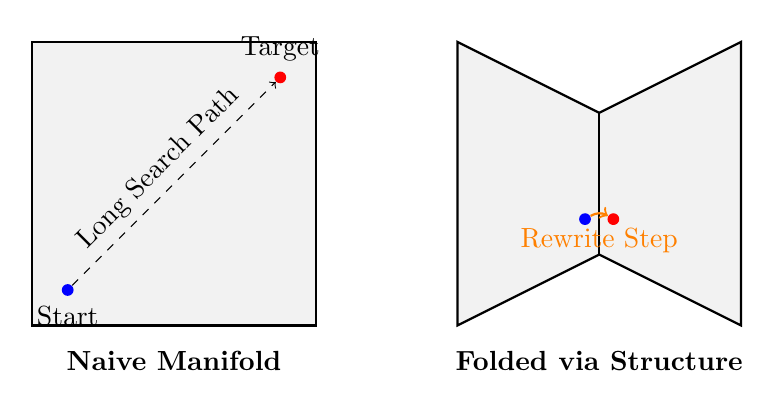
\begin{tikzpicture}[scale=0.9]
    % Left: Flat Sheet (Long Distance)
    \draw[thick, fill=gray!10] (0,0) rectangle (4,4);
    \node[circle, fill=blue, inner sep=1.5pt, label=below:Start] (A) at (0.5, 0.5) {};
    \node[circle, fill=red, inner sep=1.5pt, label=above:Target] (B) at (3.5, 3.5) {};
    \draw[dashed, ->] (A) -- (B) node[midway, sloped, above] {Long Search Path};
    \node at (2, -0.5) {\textbf{Naive Manifold}};

    % Right: Folded Sheet (Shortcut)
    \begin{scope}[shift={(6,0)}]
        \draw[thick, fill=gray!10] (0,0) -- (2,1) -- (4,0) -- (4,4) -- (2,3) -- (0,4) -- cycle;
        \draw[thick] (2,1) -- (2,3); % The fold
        \node[circle, fill=blue, inner sep=1.5pt] (A2) at (1.8, 1.5) {};
        \node[circle, fill=red, inner sep=1.5pt] (B2) at (2.2, 1.5) {};
        \draw[thick, ->, orange] (A2) to[bend left] (B2);
        \node[below, orange] at (2, 1.5) {Rewrite Step};
        \node at (2, -0.5) {\textbf{Folded via Structure}};
    \end{scope}
\end{tikzpicture}
\caption{Visualizing Local Collapse: In a naive representation (left), the distance between Start and Target is vast. In a structured RMG (right), a DPO rule "folds" the space, making the Target adjacent to the Start.}
\end{figure}

\begin{center}\rule{0.5\linewidth}{0.5pt}\end{center}

\section{\textbf{10.3 --- Local NP Collapse Looks Like Surfing the Rulial Surface}}

What does this feel like in practice?

Imagine you are trying to navigate a gnarly optimization problem. The landscape is hostile: dead ends lurk behind every decision, combinatorial explosion threatens to consume your memory, and the search space is a messy, tangled web. It feels like exponential hell.

Then, you change your representation. You might restructure the data to better match the domain, rewrite the wormholes to connect relevant nodes directly, or adjust the invariants to forbid invalid states. Perhaps you flatten a complex constraint hierarchy or prune a set of rules that are generating noise.

Suddenly, the geometry shifts. The search space flattens out. The jagged peaks of complexity smooth into a gentle slope. Geodesics—optimal paths—appear where there were once only tangles. The Time Cube widens, offering you clear, unblocked futures.

That feeling of relief, that "FINALLY" moment where the solution seems to fall into place? That is \textbf{local NP collapse}. The manifold has transformed from a jagged, exponential trap into a smooth, polynomial highway. You didn't beat the concept of NP-hardness; you simply chose to inhabit a better universe.

\begin{center}\rule{0.5\linewidth}{0.5pt}\end{center}

\section{\textbf{10.4 --- Why RMG Recursion Creates Collapse Zones}}

The secret weapon of the RMG model—the feature that distinguishes it from flat graphs or standard relational models—is recursion. \textbf{RMG recursion lets you solve subproblems at the right scale.}

In a flat system, every node is a peer, meaning every interaction must be checked against every other interaction. But in an RMG, you can rewrite inside a single node, rewrite the internal logic of an edge, or rewrite entire sub-RMG blobs as single units. You can lift computation up to a high-level abstraction or lower it into the details. You can flatten nested structures when they get in the way or reorient wormholes to bypass layers of hierarchy.

When you utilize this capability, the noise of the system dies down. You encounter fewer branches because the irrelevant ones are encapsulated. You hit fewer dead ends because the structure guides you. Contradictions and illegal matches vanish because the types prevent them from forming.

In other words, \textbf{the manifold simplifies itself.} The representation collapses the search space before your algorithm even begins to traverse it.

\begin{center}\rule{0.5\linewidth}{0.5pt}\end{center}

\section{\textbf{10.5 --- DPO Rules as Search Constraints}}

We must also reconsider the role of Double-Pushout (DPO) rules. They are not just transformation instructions; they are aggressive search constraints.

A DPO rule acts as a gatekeeper. It forbids impossible worlds from ever being instantiated. It enforces invariants, ensuring that if a property holds at step $N$, it holds at step $N+1$. It prunes illegal universes and eliminates contradictions, squeezing out combinatorial waste.

A massive percentage of the exponential branches in a typical search tree exist only because flat, untyped structures allow for nonsense. They allow the system to explore states that should never exist. Typed DPO removes this nonsense at the root. You do not wander into absurd universes because the wormholes simply refuse to open.

\textbf{NP collapses when your ruleset prunes the hell out of the search.} It does so not by heuristics, but by strict, legal, deterministic exclusion of invalid states.

\begin{figure}[h]
\centering
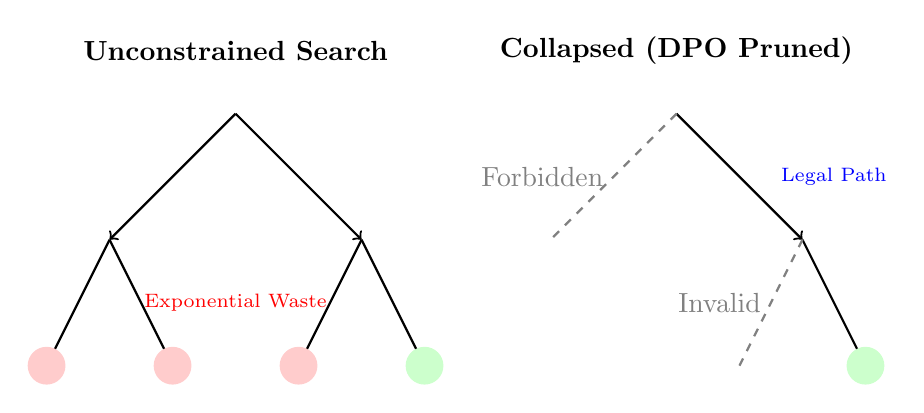
\begin{tikzpicture}[scale=0.8]
    % Jagged Search
    \node at (0, 5) {\textbf{Unconstrained Search}};
    \draw[thick, ->] (0, 4) -- (-2, 2);
    \draw[thick, ->] (0, 4) -- (2, 2);
    \draw[thick, ->] (-2, 2) -- (-3, 0);
    \draw[thick, ->] (-2, 2) -- (-1, 0);
    \draw[thick, ->] (2, 2) -- (1, 0);
    \draw[thick, ->] (2, 2) -- (3, 0);
    \fill[red!20] (-3, 0) circle (0.3); % Dead end
    \fill[red!20] (-1, 0) circle (0.3); % Dead end
    \fill[red!20] (1, 0) circle (0.3); % Dead end
    \fill[green!20] (3, 0) circle (0.3); % Goal
    \node[red, font=\scriptsize] at (0, 1) {Exponential Waste};

    % Collapsed Search
    \begin{scope}[shift={(7,0)}]
        \node at (0, 5) {\textbf{Collapsed (DPO Pruned)}};
        \draw[thick, ->] (0, 4) -- (2, 2);
        \draw[thick, dashed, gray] (0, 4) -- (-2, 2) node[midway, left] {Forbidden};
        \draw[thick, ->] (2, 2) -- (3, 0);
        \draw[thick, dashed, gray] (2, 2) -- (1, 0) node[midway, left] {Invalid};
        \fill[green!20] (3, 0) circle (0.3); % Goal
        \node[blue, font=\scriptsize] at (2.5, 3) {Legal Path};
    \end{scope}
\end{tikzpicture}
\caption{The Impact of DPO Constraints: On the left, unconstrained search explores dead ends. On the right, DPO rules forbid invalid transitions, collapsing the search into a single viable trajectory.}
\end{figure}

\begin{center}\rule{0.5\linewidth}{0.5pt}\end{center}

\section{\textbf{10.6 --- Rulial Curvature and NP Behavior Are the Same Thing}}

We now arrive at the synthesis of Part III. The big reveal is that complexity and geometry are synonyms.

\textbf{High curvature implies exponential search.}
\textbf{Low curvature implies polynomial search.}

You are literally surfing the manifold of complexity. If you inhabit a jagged area of Rulial Space, where constraints clash and invariants overlap, the wormholes will fail to connect. The Time Cube will shrink, dead ends will multiply, and the search will explode.

However, if you navigate to a smooth area of the manifold, where constraints align and invariants reinforce one another, the wormholes interlock perfectly. The Time Cube widens, worldlines cluster together, and the search collapses. NP is not an absolute constant of the universe. \textbf{NP is curvature.}

\begin{center}\rule{0.5\linewidth}{0.5pt}\end{center}

\section{\textbf{10.7 --- The Practical Takeaway: Sometimes You Win Because the Universe is Kind}}

This explains why certain technologies just feel better to use. It is why carefully structured APIs feel "easy," while others feel like fighting a hydra. It is why some languages feel smoother, why some systems seem to optimize themselves, and why some data models resist corruption while others crumble.

When a system works well, it is because its geometry is right. You didn't brute-force the NP-hard problem with raw compute power. You simply lived in a region of the manifold where NP collapses locally because \textbf{structure bends space}.

\begin{center}\rule{0.5\linewidth}{0.5pt}\end{center}

\section*{\textbf{FOR THE NERDS\texttrademark}}

\section{\textbf{NP Collapse is Local, Not Global}}

\textit{(A necessary disclaimer to prevent misunderstandings: this is still fully Turing-computable.)}

We must be precise. This is \textbf{not} a claim that P = NP. We are not invoking hypercomputation, quantum computing, or super-Turing capabilities.

We are describing \textbf{local polynomial behavior inside a structured rewrite manifold that prunes impossible universes.} Formally, this means the diameter of the reduction graph shrinks, the branching factor of the search collapses, and Rulial Distance contracts. Geodesics come to dominate the traversal. This is nothing metaphysical. It is everything computable.

\textit{(End sidebar.)}

\begin{center}\rule{0.5\linewidth}{0.5pt}\end{center}

\section{\textbf{10.8 --- Transition: From Collapse to Bundles}}

Now that you understand curvature and why NP collapses locally, you are ready to encounter the next strange phenomenon of this architecture: \textbf{Rewrite Bundles}.

These are groups of possible futures that behave like superposed alternatives, existing simultaneously until the scheduler commits to one path. Again: \textbf{Not} quantum. \textbf{Not} woo. \textbf{Not} mystical. Just structured nondeterminism bundled by adjacency.

Chapter 11 is where we formalize that.
